\documentclass[12pt, a4paper,DIV=12, bibliography=totocnumbered]{scrartcl}
\usepackage[ngerman]{babel}  
\usepackage[utf8]{inputenc}  
\usepackage[dvipsnames]{xcolor}
\usepackage{colortbl}
\usepackage{enumitem}
\usepackage{lmodern}
\usepackage{fancyhdr}
\usepackage{graphicx}
\usepackage{subfig}
\usepackage{lipsum}
\usepackage{float}
\usepackage{amsmath}
%\usepackage{upgreek}
\usepackage{framed,color}
%\usepackage{geometry}
%\usepackage[onehalfspacing]{setspace}
\usepackage{siunitx}
\sisetup{detect-weight=true, detect-family=true, locale=DE,range-phrase={\,\text{bis}\,}, list-final-separator={\,\linebreak[0] \text{und}\,},separate-uncertainty=true,per-mode=symbol-or-fraction}
\usepackage{wrapfig}
\usepackage{pdfpages}
%\usepackage{subfigure}
\usepackage{caption}
\usepackage{multirow}
\usepackage{tikz-qtree}
\usetikzlibrary{shapes.misc, positioning}
\usetikzlibrary{arrows.meta,bending}

\newcommand{\ASSNR}{1}
\newcommand{\AuthorONE}{Kamil Bannasch}
\newcommand{\MatNoONE}{405231}
\newcommand{\AuthorTWO}{Fynn Castor}
\newcommand{\MatNoTWO}{540055}



\usepackage{listings}
\usepackage{xcolor}

\definecolor{codegreen}{rgb}{0,0.6,0}
\definecolor{codegray}{rgb}{0.5,0.5,0.5}
\definecolor{codepurple}{rgb}{0.58,0,0.82}
\definecolor{backcolour}{rgb}{0.95,0.95,0.92}

\lstdefinestyle{mystyle}{
    backgroundcolor=\color{backcolour},   
    commentstyle=\color{codegreen},
    keywordstyle=\color{magenta},
    numberstyle=\tiny\color{codegray},
    stringstyle=\color{codepurple},
    basicstyle=\ttfamily\footnotesize,
    breakatwhitespace=false,         
    breaklines=true,                 
    captionpos=b,                    
    keepspaces=true,                 
    numbers=left,                    
    numbersep=5pt,                  
    showspaces=false,                
    showstringspaces=false,
    showtabs=false,                  
    tabsize=2
}
\lstset{style=mystyle}
\pagestyle{fancy}
\lhead{\slshape Assignment \ASSNR}
\rhead{\slshape\today}
\lfoot{\textsl{\AuthorONE,\AuthorTWO}}
\cfoot{ }
\rfoot{Seite \thepage}

\begin{document}
\begin{titlepage}
   \begin{center}
       \vspace*{5cm}

       \textbf{\Huge{Assignment \ASSNR}}

       \vspace{0.5cm}
        for {\large\textbf{Deep Reinforcement Learning WS2024}}
        \vspace{0.75cm}

       by \\
        \textbf{\AuthorONE}\\
        \vspace{0.125cm}
       	\textbf{\MatNoONE}\\ 
       	\vspace{0.25cm}
        \textbf{\AuthorTWO}\\
        \vspace{0.125cm}
       	\textbf{\MatNoTWO}\\ 
       	\vspace{0.25cm}
       the \textbf{\today}

       \vfill
    
    
            
   \end{center}
\end{titlepage}

\section{Excercise 1.}
\subsection{Excercise 1a.}
It seems that the code is working.  Due to the rather large pick of $\epsilon = 0.5$ the algorithm does not really take advantage of the early exploration and 
is around $60\%$ of best arm chosen. Which falls in line with the expected limit for this value of $50\%+50\%\cdot\frac{1}{4}=62.5\%$.
\begin{figure}[h]
\subfloat{
    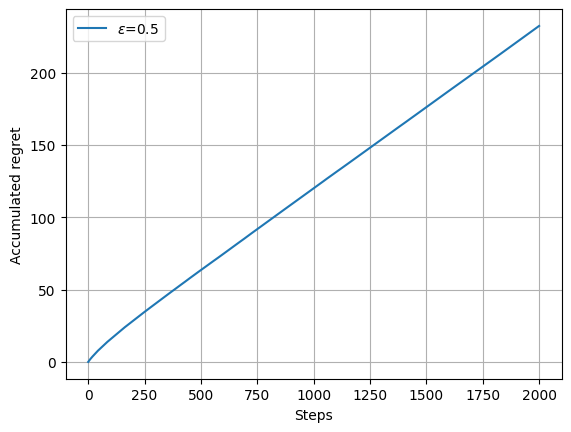
\includegraphics[width=0.45\linewidth]{graphs/1a_reg.png}}\hfill
\subfloat{
    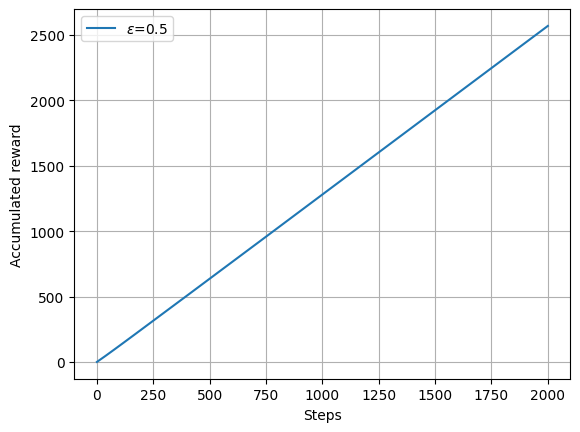
\includegraphics[width=0.45\linewidth]{graphs/1a_rew.png}}\par
\subfloat{
    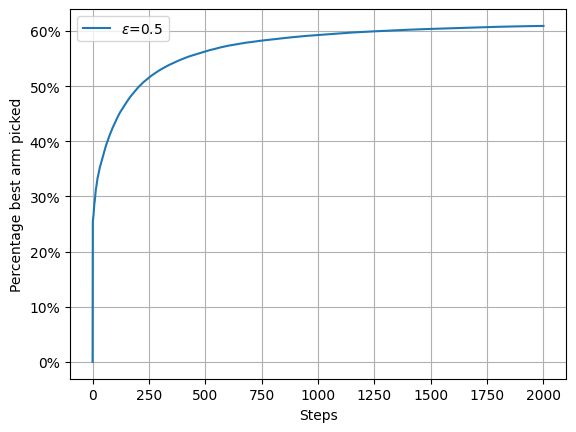
\includegraphics[width=0.45\linewidth]{graphs/1a_rel.png}}
\caption{Regret, reward, and percentage of best arm chosen for 
    4-armed bandit with normal arm distribution, where $(\mu,\sigma)\in\{(1,0.2),(1.2,0.4)(1.1,0.6),(1.4,0.8)\}$, averaged of 1000 trials}
\end{figure}

\subsection{Excercise 1b.}
As said in the ex. 1a for $\epsilon=0.5$ the algorithm can't really exploit it's early exploration due to half of the actions being picked at random.
For $\epsilon=0.01$ the algorithm suffers from the lack of early exploration and only manages to catch to the regret of $\epsilon=0.5$ after 1500 steps,
while still being outperformed by $\epsilon=0.1$ and $\epsilon=0.05$, which both seem to have an appropiate balance between exploaration and exploation, with $\epsilon=0.1$
having slightly better performance.
\begin{figure}[h]
\subfloat{
    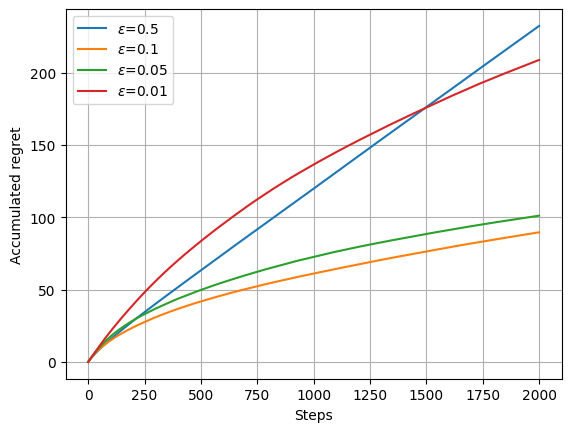
\includegraphics[width=0.45\linewidth]{graphs/1b_reg.png}}\hfill
\subfloat{
    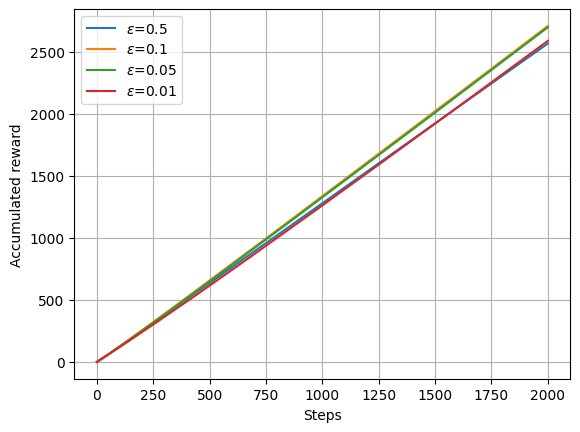
\includegraphics[width=0.45\linewidth]{graphs/1b_rew.png}}\par
\subfloat{
    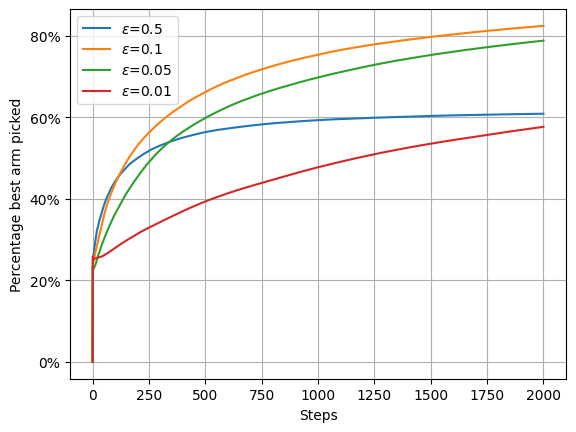
\includegraphics[width=0.45\linewidth]{graphs/1b_rel.png}}
\caption{Regret, reward, and percentage of best arm chosen for 
    4-armed bandit with normal arm distribution, where $(\mu,\sigma)\in\{(1,0.2),(1.2,0.4)(1.1,0.6),(1.4,0.8)\}$, averaged of 1000 trials, with $\epsilon \in \{0.5,0.1,0.05,0.01\}$}
\end{figure}

\newpage
\subsection{Excercise 1c.}
Due to \[Q_1(a)=Q_0(a)+\frac{1}{1}(R-Q_0(a))=R\] an overly optimistic estimate of the arm means taken as $Q_0(a)$ 
forces the algorithm to continue exploring during its greedy actions until all actions have been taken at least once.
This in turn leads to some early exploration of each action, without having to make a tradeoff in regards to the choice of $\epsilon$. 
Unfortunately due to the only small differnces in mean and the compared to that bigger $\sigma\text{'s}$ it does not have an immense impact

\subsection{Excercise 1c.}
As function a function for $\epsilon$ deterioration we chose the exponential function $f(n)=\epsilon_0e^{-\lambda\cdot n}$. 
The parameter $\epsilon_0$ hereby provides our starting $\epsilon$ whereass $\lambda$ controls the speed of deterioration. 
We found this function on wikipedia after our initial idea of using the multiplicative inverse of sigmoid function was not overly successful.
As a benchmark we used the best perform $\epsilon=0.1$ from ex 1b. One can see in the graphs that the choice of $\lambda$ has an immense impact on the 
performance of the algorithm. If it's chosen too large the algorithm gets to greedy immediately and does not explore anymore. 
On the other hand a too small value does not exploit early enough. In the end our previous benchmark was quite clearly outperformed by $\lambda=0.01$
\begin{figure}[h]
\subfloat{
    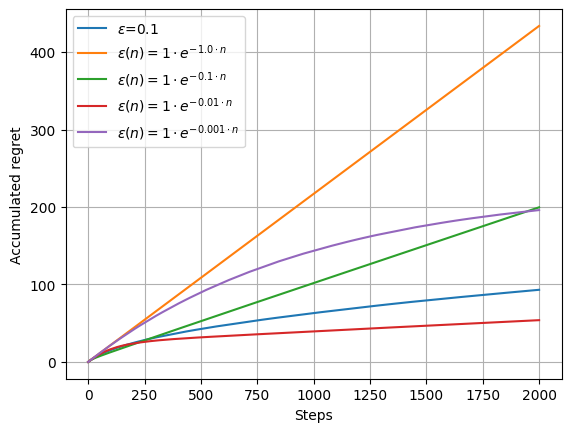
\includegraphics[width=0.45\linewidth]{graphs/1d_reg.png}}\hfill
\subfloat{
    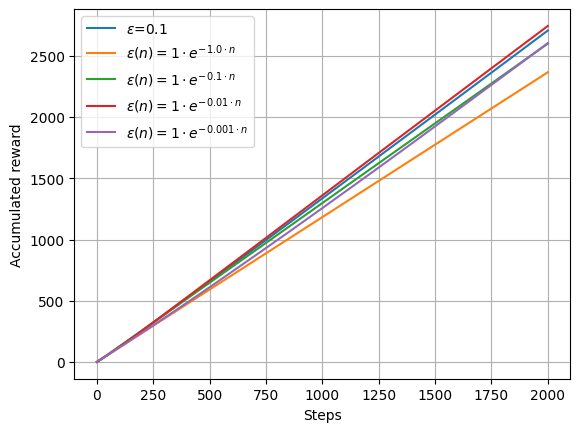
\includegraphics[width=0.45\linewidth]{graphs/1d_rew.png}}\par
\subfloat{
    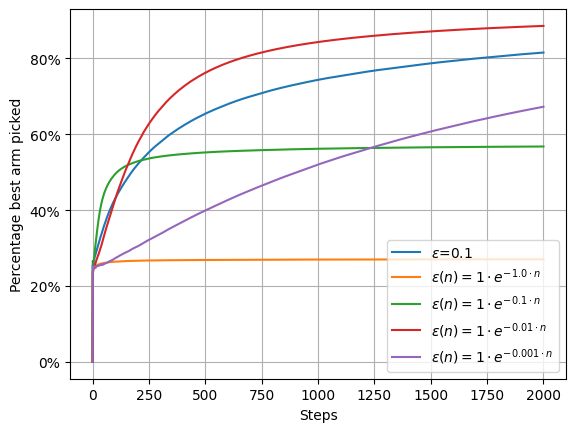
\includegraphics[width=0.45\linewidth]{graphs/1d_rel.png}}
\caption{Regret, reward, and percentage of best arm chosen for 
    4-armed bandit with normal arm distribution, where $(\mu,\sigma)\in\{(1,0.2),(1.2,0.4)(1.1,0.6),(1.4,0.8)\}$, averaged for 1000 trials}
\end{figure}
\section{Excercise 2a}
Ein k-armiger nicht stationärer Bandit ist ein Problem zur Entscheidungsfindung beim Machine
Learning. Dabei gibt es k einarmige Banditen, welche jeweils eine eigene
Wahrscheinlichkeitsverteilung für ihren Reward geben.
Im Gegensatz zu dem stationärem Bandit bleibt jedoch die Wahrscheinlichkeitsverteilung für den
Reward nicht immer gleich, sondern ändert sich im Laufe der Zeit. Bei der Modellierung eines
solchen Problems ist also darauf zu achten, dass die Verteilungen der Rewards sich im Laufe der
Zeit irgendwie ändern müssen. Das kann durch viele verschiedene Möglichkeiten dargestellt
werden, die deterministisch oder stochastisch sind. Ein Beispiel ist, dass für eine Normalverteilung
an zufällig ausgewählten Zeitpunkten der Erwartungswert geändert wird. Um einen Algorithmus
also von einem stationären auf einen nicht stationären anzupassen muss die Veränderung der
Wahrscheinlichkeiten mit berücksichtigt werden. Dafür wird im Normalfall der Algorithmus so
ummodelliert, dass neue Erkentnisse eine höhere Gewichtung haben, da es wahrscheinlicher ist,
dass diese die aktuellen Verteilungen besser erfassen als weiter zurück liegende Erkentnisse. Ein
Beispiel dafür ist bei dem Upper Confidence Bound ein Fenster zu nutzen, welches nur die letzten n
Läufe berücksichtigt. Dadurch würden weiter als n zurückliegende Ergebnisse nicht den Reward
"verfälschen". Ähnlich wie bei einem stationären Banditen sind auch bei einem nicht stationären
Banditen sowohl Ausbeutung, als auch Erkundung relevant um einerseits auf optimalen bisher
bekannten Rewards zu bleiben und andererseits mögliche bessere Rewards zu finden. Ausbeutung
kann jedoch im Vergleich zu dem stationären Banditen deutlich schlechtere Ergebnisse liefern, da
sich die Verteilung der Rewards ändern können und diese so länger auf schlechten Rewards bleiben
können. Hier ist besonders wichtig dann einen Algorithmus zu finden, welcher erkennt, wann
Erkundung eingesetzt werden sollte um die möglichst optimalen Banditen zu finden und um
möglicherweise deutlich schlechter gewordene Banditen zu verlassen. Auch hier kann wieder ein
Ansatz genutzt werden, dass länger zurückliegende Erkentnisse irrelevanter werden. Bei der
Auswertung eines solchen Algorithmus können dann wie beim stationären Banditen auch Regret
und der Cummulative Reward als Kriterien genutzt werden. Allerdings kommen bei nicht
stationären Banditen noch zusätzliche Kriterien hinzu. Einerseits die Stabilität gegenüber
Veränderungen in den Wahrscheinlichkeitsverteilungen, die möglichst hoch sein sollte und
andererseits die Reaktionsgeschwindigkeit auf Veränderungen, die möglichst schnell sein sollte
\end{document}